\documentclass[12pt]{article}
\usepackage[margin=1in]{geometry}
\usepackage{epsfig}
\usepackage{amsfonts}
\usepackage[mathcal]{euscript} 
\usepackage[tbtags]{amsmath}
\usepackage{amssymb}
\usepackage{mathrsfs}
\usepackage{import}
\usepackage{hyperref}
\usepackage{enumerate}
\usepackage{blkarray}

\renewcommand{\P}{\mathbb{P}}

\newcommand{\example}[3]{%
    \vspace{.15in}

    \noindent \textbf{Example~#1}\nopagebreak

    \noindent #2

    \noindent \textbf{Solution}: #3
}


\DeclareMathOperator*{\argmax}{\mathrm{argmax}}
\title{HMMs and the forward-backward algorithm}
\author{Ramesh Sridharan\thanks{Contact: \mbox{rameshvs@csail.mit.edu}}}
\date{}

\begin{document}
    \maketitle
    These notes give a short review of Hidden Markov Models (HMMs) and the
    forward-backward algorithm. They're written assuming familiarity with
    the sum-product belief propagation algorithm, but should be accessible
    to anyone who's seen the fundamentals of HMMs before.

    The notation here is borrowed from Introduction to Probability by Bertsekas \& Tsitsiklis: random variables are represented with capital letters, values they take are
    represented with lowercase letters, 
    $p_X$ represents a probability distribution for random variable $X$, and $p_X(x)$
    represents the probability of value $x$ (according to $p_X$).

    \section*{Hidden Markov Models}
    Figure~\ref{fig:hmm} shows the (undirected) graphical model for
    HMMs. Here's a quick recap of the important facts:
    \begin{figure}[htpb]
        \centering
        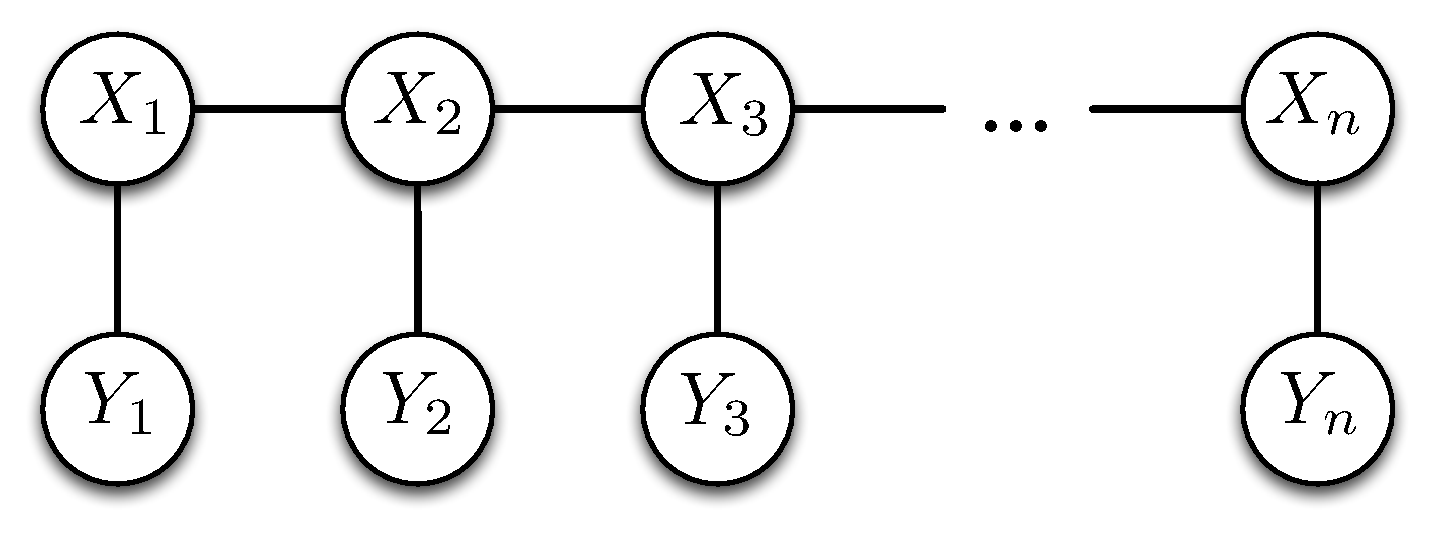
\includegraphics[width=3in]{figs/hmm.pdf}
        \caption{An undirected graphical model for the HMM. Connections
            between nodes indicate dependence.}
        \label{fig:hmm}
    \end{figure}
    \begin{itemize}
        \item We observe $Y_1$ through $Y_n$, which we model as being observed
            from hidden states $X_1$ through $X_n$.
        \item Any particular state variable $X_k$ depends only on $X_{k-1}$
            (what came before it), $X_{k+1}$ (what comes after it), and $Y_k$ (the
            observation associated with it).
        \item The goal of the forward-backward algorithm is to find the
            conditional distribution over hidden states given the data.
        \item In order to specify an HMM, we need three pieces:
            \begin{itemize}
                \item A \emph{transition distribution},
                    $p_{X_{k+1}|X_k}(x_{k+1}|x_k) = W(x_{k+1}|x_k)$~\footnote{%
                    We're only going to worry about \emph{homogeneous} Markov
                    chains, where the transition distribution doesn't change
                    over time: that's why our $W$ and $A$ notations only depend
                    on the values and not the timepoints.}, which describes the
                    distribution for the next state given the current state.
                    This is often represented as a matrix that we'll call $A$.
                    Rows of $A$ correspond to the current state, columns
                    correspond to the next state, and each entry corresponds to
                    the transition probability. So, the entry at row $i$ and
                    column $j$, $A_{ij}$, is $p_{X_{k+1}|X_k}(j|i)$, or
                    equivalently $W(j|i)$.
                \item An \emph{observation distribution} (also called an
                    ``emission distribution'') $p_{Y_k|X_k}(y_k|x_k) =
                    p_{Y|X}(y_k|x_k)$~\footnote{Once again, we'll focus on
                        Markov chains where the emission distribution is the
                    same for every state.}, which
                    describes the distribution for the output given the current
                    state. We'll represent this with matrix $B$. Here, rows
                    correspond to the current state, and columns correspond to
                    the observation. So, $B_{ij} = p_{Y|X}(j|i)$: the
                    probability of observing output $j$ from state $i$ is
                    $B_{ij}$. Since the number of possible observations isn't
                    necessarily the same as the number of possible states, $B$
                    won't necessarily be square.
                \item An \emph{initial state distribution} $p_{X_1}$,
                    which describes the starting distribution over states.
                    We'll represent this with a vector called $\pi_0$, where
                    item $i$ in the vector represents $p_{X_1}(i)$.
                    \end{itemize}
            \begin{figure}
                \centering
                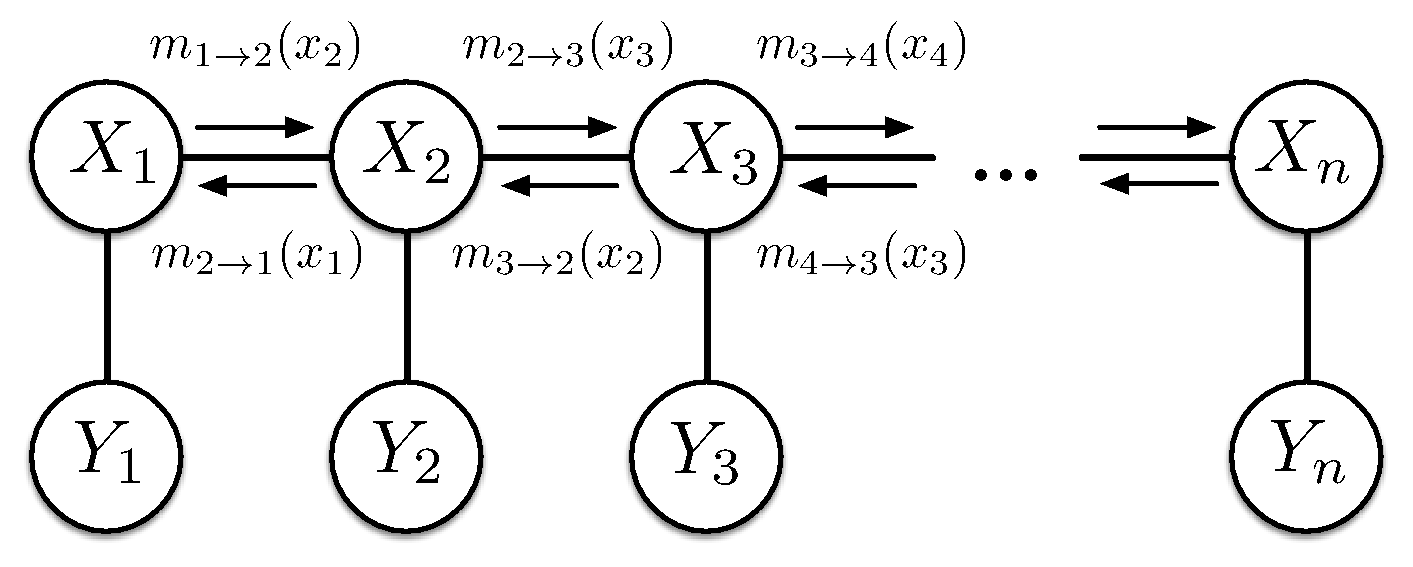
\includegraphics[width=3in]{figs/hmm-messages.pdf}
                \caption{A visualization of the forward and backward messages. Each message
                    is a table that indicates what the node at the start point believes about
                    the node at the end point.}
                \label{fig:hmm-messages}
            \end{figure}
            \vspace{-.2in}
        \item The forward-backward algorithm computes forward and backward messages as follows:
            \begin{align*}
                m_{(k-1)\to k}(x_{k}) &=
                    \sum_{x_{k-1}} 
                        \overbrace{m_{(k-2)\to (k-1)}(x_{k-1})}^{\text{prev.\ message}} 
                        \overbrace{p_{Y|X}(y_{k-1}|x_{k-1})}^{\text{observation term}} 
                        \overbrace{W(x_{k-1} | x_{k})}^{\text{transition term}} \\
                m_{(k+1)\to k}(x_{k}) &=
                    \sum_{x_{k+1}}
                        \underbrace{m_{(k+2)\to (k+1)}(x_{k+1})}_{\text{prev.\ message}} 
                        \underbrace{p_{Y|X}(y_{k+1}|x_{k+1})}_{\text{observation term}} 
                        \underbrace{W(x_{k}| x_{k+1})}_{\text{transition term}}
            \end{align*}
            These messages are illustrated in Figure~\ref{fig:hmm-messages}.
            The first forward message $m_{0 \to 1}(x_1)$ is
            initialized to $\pi_0(x_1) = p_{X_1}(x_1)$. The first backward message
            $m_{(n+1)\to n}(x_n)$ is initialized to uniform (this is equivalent to
            not including it at all).

            Figure~\ref{fig:forward-messages} illustrates the computation of one forward
            message $m_{2 \to 3}(x_3)$.
            \begin{figure}[b]
                \centering
                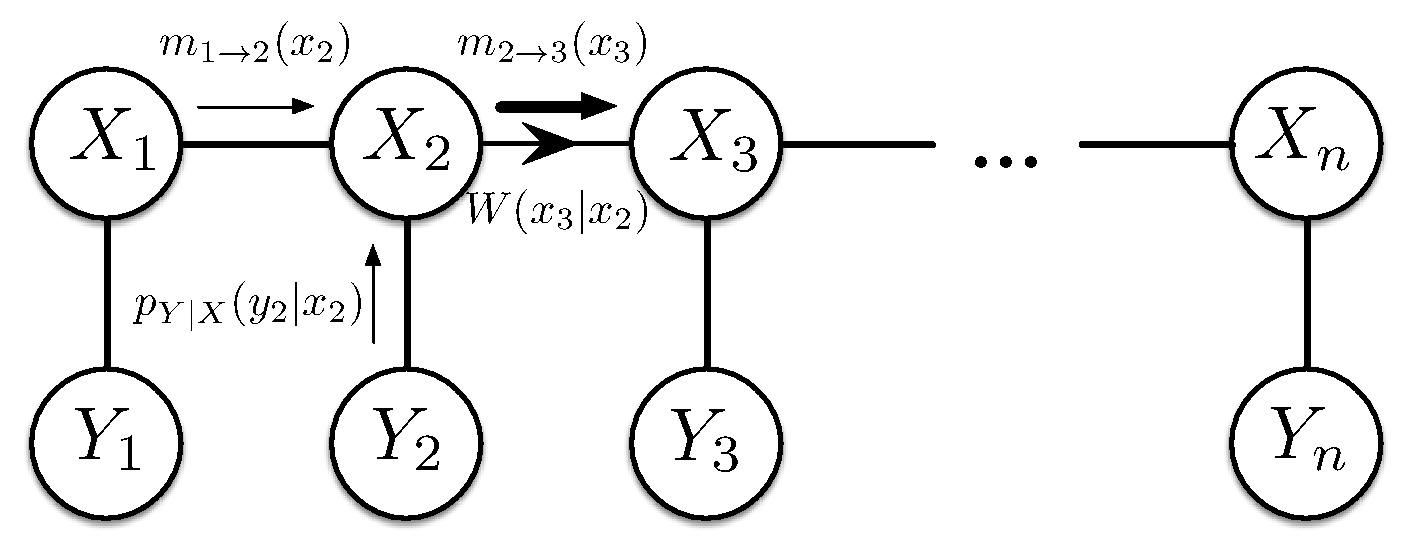
\includegraphics[width=3in]{figs/forward-message.pdf}
                \caption{An illustration of how to compute $m_{2 \to 3}(x_3)$.
                    In order for node 2 to summarize its belief about $X_3$, it
                    must incorporate the previous message $m_{1 \to 2}(x_2)$,
                    its observation $p_{Y|X}(y_2|x_2)$, and the relationship
                    $W(x_3|x_2)$ between $X_2$ and $X_3$.}
                \label{fig:forward-messages}
            \end{figure}
        \item To obtain a marginal distribution for a particular state given
            all the observations, $p_{X_k|Y_1,\ldots,Y_n}$, we simply multiply the incoming messages
            together with the observation term, and then normalize:
            \begin{align*}
                p_{X_k | Y_1, \ldots, Y_n}(x_k|y_1,\ldots,y_n) &\propto m_{(k-1)\to k}(x_{k})m_{(k+1)\to k}(x_{k}) p_{Y|X}(y_k|x_k)
            \end{align*}
            Here, the symbol $\propto$ means ``is proportional to'', and indicates that we have to
            normalize at the end so that the answer sums to 1.
        \item Traditionally, the forward-backward algorithm computes a slightly
            different set of messages. The forward message $\alpha_k$
            represents a message from $k-1$ to $k$ that includes
            $p_{Y|X}(y_k|x_k)$, and the backward message $\beta_k$ represents a
            message from $k+1$ to $k$ identical to $m_{(k+1) \to k}$ above.
            \begin{align*}
                \alpha_{k}(x_{k}) &=
                    \overbrace{p_{Y|X}(y_{k}|x_{k})}^{\text{observation term}} 
                    \sum_{x_{k-1}}
                        \overbrace{\alpha_{k-1}(x_{k-1})}^{\text{prev.\ message}}
                        \overbrace{W(x_{k-1} | x_{k})}^{\text{transition term}} \\
                \beta_{k}(x_{k}) &=
                    \sum_{x_{k+1}}
                        \underbrace{\beta_{k+1}(x_{k+1})}_{\text{prev.\ message}} 
                        \underbrace{p_{Y|X}(y_{k+1}|x_{k+1})}_{\text{observation\ term}} 
                        \underbrace{W(x_{k}| x_{k+1})}_{\text{transition term}}
            \end{align*}
            These messages have a particularly nice interpretation as probabilities:
            \begin{align*}
                \alpha_k(x_k) &= p_{Y_1, Y_2, \ldots, Y_k, X_k}(y_1, y_2, \ldots, y_k, x_k) \\
                \beta_k(x_k) &= p_{Y_{k+1}, Y_{k+2}, \ldots, Y_n| X_k}(y_{k+1}, y_{k+2}, \ldots, y_n | x_k)
            \end{align*}
            The initial forward $\alpha$ message is initialized to $\alpha_1(x_1) = p_{X_1}(x_1)p_{Y|X}(y_1|x_1)$.
            To obtain a marginal distribution, we simply multiply the messages together and
            normalize:
            \begin{align*}
                p_{X_k | Y_1, \ldots, Y_n}(x_k|y_1,\ldots,y_n) &\propto \alpha_{k}(x_{k})\beta_{k}(x_{k})
            \end{align*}
    \end{itemize}

    \example{}{%
    Suppose you send a robot to Mars.
    Unfortunately, it gets stuck in a canyon while landing and most of its sensors break.
    You know the canyon has 3 areas. Areas 1 and 3 are sunny and hot,
    while Area 2 is cold. You decide to plan
    a rescue mission for the robot from Area 3, knowing the following
    things about the robot:
    \begin{itemize}
        \item Every hour, it tries to move forward by one area (i.e.\ from Area 1 to Area 2, or Area 2 to Area 3).
            It succeeds with probability $0.75$ and fails with probability $0.25$. If it fails, it stays
            where it is. If it is in Area 3, it always stays there (and waits to be rescued).
        \item The temperature sensor still works. Every hour, we get a binary reading telling us whether the
            robot's current environment is hot or cold.
        \item We have no idea where the robot initially got stuck.
    \end{itemize}
    }{%
    \begin{enumerate}[(a)]
        \item Construct an HMM for this problem: define a transition matrix $A$, an observation matrix $B$,
            and an initial state distribution $\pi_0$.
        \item Suppose we observe the sequence (hot, cold, hot). First, before doing any computation,
           determine the sequence of locations. Then, compute the forward and backward messages,
            and determine the distribution for the second state using the messages. Do your answers
            match up?
    \end{enumerate}
    \begin{enumerate}[(a)]
        \item We'll start with the transition matrix. Remember that each row corresponds to the current
            state, and each column corresponds to the next state. We'll use 3 states, each corresponding
            to an area.
            \begin{itemize}
                \item If the robot is in Area 1, it stays where it is with probability 0.25, moves to
                    Area 2 with probability 0.75, and can't move to Area 3.
                \item Similarly, if the robot is in Area 2, it stays where it is with probability 0.25,
                    can't move back to Area 1, and moves to Area 3 with probability 0.75.
                \item If the robot is in Area 3, it always stays in Area 3.
            \end{itemize}
            Each item above gives us one row of $A$. Putting it all together, we obtain
            \begin{align*}
                A &= 
                \begin{blockarray}{cccc} & 1 & 2 & 3 \\
                    \begin{block}{c(ccc)} 
                        1 & 0.25 & 0.75 & 0    \\
                        2 & 0    & 0.25 & 0.75 \\
                        3 & 0    & 0    & 1    \\
                    \end{block}
                \end{blockarray}
            \end{align*}

            Next, let's look at the observation matrix. There are two possible
            observations, hot and cold. Areas 1 and 3 always produce ``hot''
            readings while Area 2 always produces a ``cold'' reading:
            \begin{align*}
                B  = \begin{blockarray}{ccc}
                    & \text{hot} & \text{cold} \\
                    \begin{block}{c(cc)}
                        1 & 1 & 0 \\
                        2 & 0 & 1 \\
                        3 & 1 & 0 \\
                    \end{block}
                \end{blockarray}
            \end{align*}

            Last but not least, since we have no idea where the robot starts, our initial state
            distribution will be uniform:
            \begin{align*}
                \pi_0 = 
                \begin{blockarray}{c(c)} 
                    1 & 1/3 \\
                    2 & 1/3 \\
                    3 & 1/3 \\
                \end{blockarray}
            \end{align*}

        \item Before doing any computation, we see that the sequence (hot,cold,hot) could only
            have been observed from the hidden state sequence (1,2,3). Make sure you convince
            yourself this is true before continuing!

            We'll start with the forward messages.
            \begin{align*}
                m_{1 \to 2} &= \sum_{x_1} \underbrace{m_{0 \to 1}(x_1) p_{Y|X}(y_1|x_1)}_{\text{depends only on $x_1$ and $y_1$}} \psi(x_1,x_2)
            \end{align*}
            The output message should have three different possibilities, one for each value of $x_2$.
            We can therefore represent it as a vector indexed by $x_2$:
            \begin{align*}
                \begin{blockarray}{cc}
                    \begin{block}{(c)c}
                        \cdot & \text{value for $x_2 = 1$} \\
                        \cdot & \text{value for $x_2 = 2$} \\
                        \cdot & \text{value for $x_2 = 3$} \\
                    \end{block}
                \end{blockarray}
            \end{align*}
            For each term in the sum (i.e., each possible value of $x_1$):
            \begin{itemize}
                \item $m_{0 \to 1}$ comes from from the initial distribution. Normally it would come from
                    the previous message, but our first forward message is always set to
                    initial state distribution.
                \item $p_{Y|X}(y_1|x_1)$ comes from the column of $B$ corresponding
                    to our observation $y_1 = $ hot.
                \item $\psi$ comes from a row of $A$: we are fixing $x_1$ and
                    asking about possible values for $x_2$, which corresponds
                    exactly to the transition distributions given in the rows
                    of $A$ (remember that the rows of $A$ correspond to the
                    current state and the columns correspond to the next
                    state).
            \end{itemize}
            So, we obtain
            \begin{align*}
                m_{1 \to 2} &=
                \overbrace{\frac{1}{3} \cdot 1 \cdot \begin{pmatrix} .25 \\ .75 \\ 0 \end{pmatrix}}^{x_1 = 1} +
                \overbrace{\frac{1}{3} \cdot 0 \cdot \begin{pmatrix} 0 \\ .25 \\ .75 \end{pmatrix}}^{x_1 = 2} +
                \overbrace{\frac{1}{3} \cdot 1 \cdot \begin{pmatrix} 0 \\ 0 \\ 1 \end{pmatrix}}^{x_1 = 3} \\
                &\propto \begin{pmatrix} 1 \\ 3 \\ 4 \end{pmatrix}
            \end{align*}
            Since our probabilities are eventually computed by multiplying messages and normalizing,
            we can arbitrary renormalize at any step to make the computation easier.

            For the second message, we perform a similar computation:
            \begin{align*}
                m_{2 \to 3} &= 
                    \sum_{x_2} {m_{1 \to 2}(x_2) \tilde{\phi}(x_2)} \psi(x_2,x_3) \\
                &=
                    \overbrace{1 \cdot 0 \cdot \begin{pmatrix} .25 \\ .75 \\ 0 \end{pmatrix}}^{x_2 = 1} +
                    \overbrace{3 \cdot 1 \cdot \begin{pmatrix} 0 \\ .25 \\ .75 \end{pmatrix}}^{x_2 = 2} +
                    \overbrace{4 \cdot 0 \cdot \begin{pmatrix} 0 \\ 0 \\ 1 \end{pmatrix}}^{x_2 = 3} \\
                &\propto \begin{pmatrix} 0 \\ 1 \\ 3 \end{pmatrix}
            \end{align*}


            The backwards messages are computed using a similar formula:
            \begin{align*}
                m_{3 \to 2} &= \sum_{x_3} \underbrace{m_{4 \to 3}(x_3) \tilde{\phi}(x_3)}_{\text{depends only on $x_3$}} \psi(x_2,x_3)
            \end{align*}
            The first backwards message, $m_{4 \to 3}(x_3)$, is always initialized to uniform
            since we have no information about what the last state should be. Note that this is equivalent
            to not including that term at all.

            For each value of $x_3$, the transition term $\psi(x_2,x_3)$ is now drawn from a \emph{column}
            of $A$, since we are interested in the probability of arriving at $x_3$ from each possible
            state for $x_2$. We compute the messages as:
            \begin{align*}
                m_{3 \to 2} &= 
                    \overbrace{1 \cdot \begin{pmatrix} .25 \\ 0 \\ 0 \end{pmatrix}}^{x_3 = 1} +
                    \overbrace{0 \cdot \begin{pmatrix} .75 \\ .25 \\ 0 \end{pmatrix}}^{x_3 = 2} +
                    \overbrace{1 \cdot \begin{pmatrix} 0 \\ .75 \\ 1 \end{pmatrix}}^{x_3 = 3} \\
                &\propto \begin{pmatrix} 1 \\ 3 \\ 4 \end{pmatrix}
            \end{align*}

            Similarly, the second backwards message is:
            \begin{align*}
                m_{2 \to 1} &= 
                \overbrace{1 \cdot 0 \cdot \begin{pmatrix} .25 \\ 0 \\ 0 \end{pmatrix}}^{x_2 = 1} +
                \overbrace{3 \cdot 1 \cdot \begin{pmatrix} .75 \\ .25 \\ 0 \end{pmatrix}}^{x_2 = 2} +
                \overbrace{4 \cdot 0 \cdot \begin{pmatrix} 0 \\ .75 \\ 1 \end{pmatrix}}^{x_2 = 3} \\
                &\propto \begin{pmatrix} 3 \\ 1 \\ 0 \end{pmatrix}
            \end{align*}

            Notice from the symmetry of the problem that our forwards messages and backwards messages
            were the same.

            To compute the marginal distribution for $X_2$ given the data, we multiply the messages and
            the observation:
            \begin{align*}
                p_{X_2 | Y_1, \ldots, Y_n}(x_2|y_1,\ldots,y_n) &\propto 
                    m_{1 \to 2}(x_2) 
                    m_{3 \to 2}(x_2) 
                    \tilde{\phi}(x_2) \\
                &\propto
                    \begin{pmatrix} 1 \\ 3 \\ 4 \end{pmatrix} \cdot
                    \begin{pmatrix} 1 \\ 3 \\ 4 \end{pmatrix} \cdot
                    \begin{pmatrix} 0 \\ 1 \\ 0 \end{pmatrix} \\
                &= \begin{pmatrix} 0 \\ 1 \\ 0 \end{pmatrix} \\
            \end{align*}
            Notice that in this case, because of our simplified observation model, the observation ``cold''
            allowed us to determine the state. This matches up with our earlier conclusion that the robot
            must have been in Area 2 during the second hour.

            If we were to compute $\alpha$ messages, we would start with our
            initial message, $\alpha_1$:
            \begin{align*}
                \alpha_1(x_1) &= p_{X_1}(x_1) p_{Y|X}(y_1|x_1) = \begin{pmatrix} 1/3 \\ 0 \\ 1/3 \end{pmatrix} \\
            \end{align*}

            The first real message is computed as follows:
            \begin{align*}
                \alpha_{2} &=
                \begin{pmatrix} 0 \\ 1 \\ 0 \end{pmatrix} \cdot \left(
                \overbrace{\cdot 1/3 \cdot \begin{pmatrix} .25 \\ .75 \\ 0 \end{pmatrix}}^{x_1 = 1} +
                \overbrace{\cdot 0 \cdot \begin{pmatrix} 0 \\ .25 \\ .75 \end{pmatrix}}^{x_1 = 2} +
                \overbrace{\cdot 1/3 \cdot \begin{pmatrix} 0 \\ 0 \\ 1 \end{pmatrix}}^{x_1 = 3}\right) \\
                &\propto \begin{pmatrix} 0 \\ 1 \\ 0 \end{pmatrix}
            \end{align*}

            The second message is similar:
            \begin{align*}
                \alpha_{3} &=
                \begin{pmatrix} 1 \\ 0 \\ 1 \end{pmatrix} \cdot \left(
                \overbrace{\cdot 0 \cdot \begin{pmatrix} .25 \\ .75 \\ 0 \end{pmatrix}}^{x_1 = 1} +
                \overbrace{\cdot 1 \cdot \begin{pmatrix} 0 \\ .25 \\ .75 \end{pmatrix}}^{x_1 = 2} +
                \overbrace{\cdot 0 \cdot \begin{pmatrix} 0 \\ 0 \\ 1 \end{pmatrix}}^{x_1 = 3}\right) \\
                &\propto \begin{pmatrix} 1 \\ 0 \\ 1 \end{pmatrix}
            \end{align*}

            The $\beta$ messages would be identical to our backwards messages computed earlier.
    \end{enumerate}
}
\end{document}
